\begin{tikzpicture}[scale=0.8,>=stealth]
% landscape: R(x) on unit circle, min/max at eigenvectors
\draw[->] (-2.6,0)--(2.6,0) node[right]{$x_1$};
\draw[->] (0,-2.6)--(0,2.6) node[above]{$x_2$};
\draw (0,0) circle (2.2);
\foreach \r in {0.6,1.1,1.6,2.1} \draw[blue!60,rotate=25] (0,0) ellipse ({\r*1.7} and {\r*0.55});
\draw[->,thick,red] (0,0)--({2.2*cos(25)},{2.2*sin(25)}) node[right=2pt]{$\mathbf q_1$: $R=\lambda_1$};
\draw[->,thick,red] (0,0)--({-2.2*sin(25)},{2.2*cos(25)}) node[above=2pt]{$\mathbf q_2$: $R=\lambda_2$};
\node at (0,-3.1) {$R(x)=\dfrac{x^{T}Ax}{x^{T}x}$ extremized at eigenvectors};
\end{tikzpicture}
